% ═══════════════════════════════════════════════════════════════════════════
%  DDF — préambule commun aux sept articles.  % ═══════════════════════════════════════════════════════════════════════════
%  DDF — préambule commun aux sept articles.  % ═══════════════════════════════════════════════════════════════════════════
%  DDF — préambule commun aux sept articles.  \input{ddf-common} en tête.
%  Définit : la mise en page, les macros, le bloc de série, la déclaration
%  d'usage d'outils, et le bloc de traçabilité.
% ═══════════════════════════════════════════════════════════════════════════
\documentclass[11pt,a4paper]{article}
\usepackage[margin=2.3cm]{geometry}
\usepackage{amsmath,amssymb,booktabs,hyperref,graphicx,xcolor}
\usepackage[expansion=false]{microtype}
\hypersetup{colorlinks=true,linkcolor=blue!45!black,citecolor=blue!45!black,urlcolor=blue!45!black}

% ---------- macros physiques ----------
\newcommand{\MPl}{M_{\rm Pl}}\newcommand{\Mred}{\bar M_{\rm Pl}}
\newcommand{\Mfive}{M_5}\newcommand{\MS}{M_S}\newcommand{\V}{\mathcal V}
\newcommand{\Neff}{N_{\rm eff}}\newcommand{\cb}{c_b}\newcommand{\ab}{\alpha_b}

% ---------- étiquettes épistémiques ----------
\newcommand{\Derived}{\textit{[Derived]}}
\newcommand{\Input}{\textit{[Input, natural]}}
\newcommand{\Posited}{\textit{[Posited]}}
\newcommand{\Candidate}{\textit{[Candidate]}}
\newcommand{\Open}{\textit{[Open, declared]}}
\newcommand{\Verified}{\textit{[Verified]}}

% ---------- bloc de série : \seriesdate{III}{The medium} ----------
\newcommand{\seriesdate}[2]{%
 \date{\small \textit{Cosmic Shadow Geometry} \\ \small Article #1 of VII
 \,\textperiodcentered\, #2 \,\textperiodcentered\, \today}}

% ---------- déclaration d'outils, identique dans les sept ----------
\newcommand{\toolsstatement}{%
\section*{Declaration on computational tools}
\addcontentsline{toc}{section}{Declaration on computational tools}
\small
This work was carried out by the author alone, without institutional affiliation.
\textbf{Large language models were used as computational and analytical assistants
throughout}: to write and debug the numerical scripts, to run the scans and
minimisations, to produce the figures, to check algebra and dimensional
consistency, to search and summarise the literature, and to audit drafts for
internal contradictions. Several distinct systems were used and cross-checked
against one another; no single system's output was accepted without an
independent numerical or analytical verification.

\textbf{The author is solely responsible for the physical hypotheses, the
interpretation of every result, the epistemic labels attached to each claim, and
the decision of what to publish and what to withdraw.} All quantitative
statements in this paper are reproduced by the scripts listed in the
traceability section; a reader who runs them obtains the numbers printed here
without needing any language model. Where an earlier draft contained an error
introduced by an unverified computation, it is recorded as a withdrawal rather
than silently removed.
\normalsize}

% ---------- bloc de traçabilité : \traceability{V}{...} ----------
\newcommand{\traceability}[2]{%
\section*{Data availability, traceability and reproducibility}
\addcontentsline{toc}{section}{Traceability}
\small
Every number, table and figure in this paper is regenerated by the scripts of
this article's folder. The complete repository ---sources, scripts, proof files,
figures and compiled documents for all seven articles--- is at
\url{https://github.com/HBoufourou}.

\textbf{Folder \texttt{article-#1/} contains:}
\begin{itemize}\itemsep2pt
\item \texttt{tex/} --- the \LaTeX\ source and the shared preamble \texttt{ddf-common.tex};
\item \texttt{scripts/} --- every computation, each runnable standalone with
      \texttt{python3 <name>.py} and printing its own verification verdict;
\item \texttt{proofs/} --- the JSON files carrying the certified values.
      \textbf{Any number absent from \texttt{proofs/} is not certified};
\item \texttt{data/} --- the CSV tables underlying the figures;
\item \texttt{figures/} --- the PNG files, regenerated by \texttt{scripts/figures.py};
\item \texttt{pdf/} --- the compiled article;
\item \texttt{VERIFICATION.txt} --- the output of the verification suite.
\end{itemize}
#2
\normalsize}
 en tête.
%  Définit : la mise en page, les macros, le bloc de série, la déclaration
%  d'usage d'outils, et le bloc de traçabilité.
% ═══════════════════════════════════════════════════════════════════════════
\documentclass[11pt,a4paper]{article}
\usepackage[margin=2.3cm]{geometry}
\usepackage{amsmath,amssymb,booktabs,hyperref,graphicx,xcolor}
\usepackage[expansion=false]{microtype}
\hypersetup{colorlinks=true,linkcolor=blue!45!black,citecolor=blue!45!black,urlcolor=blue!45!black}

% ---------- macros physiques ----------
\newcommand{\MPl}{M_{\rm Pl}}\newcommand{\Mred}{\bar M_{\rm Pl}}
\newcommand{\Mfive}{M_5}\newcommand{\MS}{M_S}\newcommand{\V}{\mathcal V}
\newcommand{\Neff}{N_{\rm eff}}\newcommand{\cb}{c_b}\newcommand{\ab}{\alpha_b}

% ---------- étiquettes épistémiques ----------
\newcommand{\Derived}{\textit{[Derived]}}
\newcommand{\Input}{\textit{[Input, natural]}}
\newcommand{\Posited}{\textit{[Posited]}}
\newcommand{\Candidate}{\textit{[Candidate]}}
\newcommand{\Open}{\textit{[Open, declared]}}
\newcommand{\Verified}{\textit{[Verified]}}

% ---------- bloc de série : \seriesdate{III}{The medium} ----------
\newcommand{\seriesdate}[2]{%
 \date{\small \textit{Cosmic Shadow Geometry} \\ \small Article #1 of VII
 \,\textperiodcentered\, #2 \,\textperiodcentered\, \today}}

% ---------- déclaration d'outils, identique dans les sept ----------
\newcommand{\toolsstatement}{%
\section*{Declaration on computational tools}
\addcontentsline{toc}{section}{Declaration on computational tools}
\small
This work was carried out by the author alone, without institutional affiliation.
\textbf{Large language models were used as computational and analytical assistants
throughout}: to write and debug the numerical scripts, to run the scans and
minimisations, to produce the figures, to check algebra and dimensional
consistency, to search and summarise the literature, and to audit drafts for
internal contradictions. Several distinct systems were used and cross-checked
against one another; no single system's output was accepted without an
independent numerical or analytical verification.

\textbf{The author is solely responsible for the physical hypotheses, the
interpretation of every result, the epistemic labels attached to each claim, and
the decision of what to publish and what to withdraw.} All quantitative
statements in this paper are reproduced by the scripts listed in the
traceability section; a reader who runs them obtains the numbers printed here
without needing any language model. Where an earlier draft contained an error
introduced by an unverified computation, it is recorded as a withdrawal rather
than silently removed.
\normalsize}

% ---------- bloc de traçabilité : \traceability{V}{...} ----------
\newcommand{\traceability}[2]{%
\section*{Data availability, traceability and reproducibility}
\addcontentsline{toc}{section}{Traceability}
\small
Every number, table and figure in this paper is regenerated by the scripts of
this article's folder. The complete repository ---sources, scripts, proof files,
figures and compiled documents for all seven articles--- is at
\url{https://github.com/HBoufourou}.

\textbf{Folder \texttt{article-#1/} contains:}
\begin{itemize}\itemsep2pt
\item \texttt{tex/} --- the \LaTeX\ source and the shared preamble \texttt{ddf-common.tex};
\item \texttt{scripts/} --- every computation, each runnable standalone with
      \texttt{python3 <name>.py} and printing its own verification verdict;
\item \texttt{proofs/} --- the JSON files carrying the certified values.
      \textbf{Any number absent from \texttt{proofs/} is not certified};
\item \texttt{data/} --- the CSV tables underlying the figures;
\item \texttt{figures/} --- the PNG files, regenerated by \texttt{scripts/figures.py};
\item \texttt{pdf/} --- the compiled article;
\item \texttt{VERIFICATION.txt} --- the output of the verification suite.
\end{itemize}
#2
\normalsize}
 en tête.
%  Définit : la mise en page, les macros, le bloc de série, la déclaration
%  d'usage d'outils, et le bloc de traçabilité.
% ═══════════════════════════════════════════════════════════════════════════
\documentclass[11pt,a4paper]{article}
\usepackage[margin=2.3cm]{geometry}
\usepackage{amsmath,amssymb,booktabs,hyperref,graphicx,xcolor}
\usepackage[expansion=false]{microtype}
\hypersetup{colorlinks=true,linkcolor=blue!45!black,citecolor=blue!45!black,urlcolor=blue!45!black}

% ---------- macros physiques ----------
\newcommand{\MPl}{M_{\rm Pl}}\newcommand{\Mred}{\bar M_{\rm Pl}}
\newcommand{\Mfive}{M_5}\newcommand{\MS}{M_S}\newcommand{\V}{\mathcal V}
\newcommand{\Neff}{N_{\rm eff}}\newcommand{\cb}{c_b}\newcommand{\ab}{\alpha_b}

% ---------- étiquettes épistémiques ----------
\newcommand{\Derived}{\textit{[Derived]}}
\newcommand{\Input}{\textit{[Input, natural]}}
\newcommand{\Posited}{\textit{[Posited]}}
\newcommand{\Candidate}{\textit{[Candidate]}}
\newcommand{\Open}{\textit{[Open, declared]}}
\newcommand{\Verified}{\textit{[Verified]}}

% ---------- bloc de série : \seriesdate{III}{The medium} ----------
\newcommand{\seriesdate}[2]{%
 \date{\small \textit{Cosmic Shadow Geometry} \\ \small Article #1 of VII
 \,\textperiodcentered\, #2 \,\textperiodcentered\, \today}}

% ---------- déclaration d'outils, identique dans les sept ----------
\newcommand{\toolsstatement}{%
\section*{Declaration on computational tools}
\addcontentsline{toc}{section}{Declaration on computational tools}
\small
This work was carried out by the author alone, without institutional affiliation.
\textbf{Large language models were used as computational and analytical assistants
throughout}: to write and debug the numerical scripts, to run the scans and
minimisations, to produce the figures, to check algebra and dimensional
consistency, to search and summarise the literature, and to audit drafts for
internal contradictions. Several distinct systems were used and cross-checked
against one another; no single system's output was accepted without an
independent numerical or analytical verification.

\textbf{The author is solely responsible for the physical hypotheses, the
interpretation of every result, the epistemic labels attached to each claim, and
the decision of what to publish and what to withdraw.} All quantitative
statements in this paper are reproduced by the scripts listed in the
traceability section; a reader who runs them obtains the numbers printed here
without needing any language model. Where an earlier draft contained an error
introduced by an unverified computation, it is recorded as a withdrawal rather
than silently removed.
\normalsize}

% ---------- bloc de traçabilité : \traceability{V}{...} ----------
\newcommand{\traceability}[2]{%
\section*{Data availability, traceability and reproducibility}
\addcontentsline{toc}{section}{Traceability}
\small
Every number, table and figure in this paper is regenerated by the scripts of
this article's folder. The complete repository ---sources, scripts, proof files,
figures and compiled documents for all seven articles--- is at
\url{https://github.com/HBoufourou}.

\textbf{Folder \texttt{article-#1/} contains:}
\begin{itemize}\itemsep2pt
\item \texttt{tex/} --- the \LaTeX\ source and the shared preamble \texttt{ddf-common.tex};
\item \texttt{scripts/} --- every computation, each runnable standalone with
      \texttt{python3 <name>.py} and printing its own verification verdict;
\item \texttt{proofs/} --- the JSON files carrying the certified values.
      \textbf{Any number absent from \texttt{proofs/} is not certified};
\item \texttt{data/} --- the CSV tables underlying the figures;
\item \texttt{figures/} --- the PNG files, regenerated by \texttt{scripts/figures.py};
\item \texttt{pdf/} --- the compiled article;
\item \texttt{VERIFICATION.txt} --- the output of the verification suite.
\end{itemize}
#2
\normalsize}

\graphicspath{{figures/}{../figures/}}
\title{\textbf{The Dark Dimension Framework III:\\ The medium --- two roles, one response}}
\author{Hicham Boufourou\\ \small\textit{Independent Researcher, Brussels, Belgium}\\ \small\texttt{hicham.boufourou@hotmail.com}}
\seriesdate{III}{The medium}
\newcommand{\Msun}{M_{\odot}}
\begin{document}\maketitle
\begin{abstract}
\noindent Articles I and II built the stage of the Dark Dimension Framework and its tower; this article populates them and lets them act. The single bulk field $\Phi$, bound in the derived well, plays two roles set by its position on the tower. The upper levels are a particulate \emph{reservoir}: populated primordially by misalignment across the tower --- cold, never reheated, with initial fractions $0.27{:}0.39{:}0.22{:}0.12$ for the natural flat displacement, a choice labelled as such since no identity of the Airy zeros fixes it --- the reservoir carries at least $98.6\%$ of the dark mass and behaves gravitationally as cold dark matter wherever lensing or dynamics are measured. The ground level is a coherent \emph{condensate}, at most $1.4\%$ of the sector, fed continuously by a drip: direct graviton decay between levels is suppressed by $e^{-10^{24}}$, so the tower relaxes through a scalar cascade whose every step is stimulated by the reservoir's Bose degeneracy, $n\lambda_{\rm dB}^{3}\sim10^{10\text{--}12}$, computed rather than assumed; the operative self-coupling $\lambda\sim10^{-18}$ then sits six orders below the unstimulated estimate, inside a two-jawed window --- an astrophysical ceiling ($\lambda<2\times10^{-13}$, Bullet Cluster~\cite{Clowe}) over a cosmological floor. The condensate is what answers back: through the single boundary vertex of Articles I--II, with amplitude $\alpha_{b}=3.3\,c_{b}$, its phonon-mediated pull adds to gravity and reproduces the radial-acceleration relation of galaxies; and because the response requires coherence, it carries its own off-switch. Coherence dies within a radius $R_{\rm dec}=K\,(M/\Msun)^{1/3}/(f\rho)$ of any mass concentration, with the single constant $K=4.9\times10^{-4}~\mathrm{pc\cdot GeV\,cm^{-3}}$ and the condensed fraction measured to $f\in[1.2\times10^{-3},\,8.42\times10^{-3}]$: the Solar System sits inside its own decoherence bubble ($\gtrsim$30~kau at the tightest), so Cassini~\cite{Bertotti}'s $\gamma-1\lesssim2\times10^{-5}$ is met \emph{identically}, with a factor of a thousand in radius to spare and a bubble edge smoothed on the condensate's healing length; wide binaries beyond $\sim$10~kau are predicted Newtonian --- a null confirmed by Gaia DR3 at $\gamma=1.00$--$1.05$ with the modified-dynamics enhancement excluded at high significance, the difficulty of other frameworks arriving here as a verified prediction; and clusters are handled at two tiers, the first parameter-free (cluster masses are cluster masses, by mass budget alone), the second a declared scaling whose choice does not move the conclusion. Finally, the universality of the baryon--medium coupling --- long an open structural question --- is bounded by data in this article: a mass-to-light-marginalised analysis of 171 SPARC~\cite{SPARC,McGaugh16} galaxies limits any composition dependence to $|\Delta\alpha_{b}/\alpha_{b}|\leq9\%$ at the standard stellar mass-to-light ratio, and $\leq14\%$ across its plausible range, an order of magnitude above the $\sim0.7\%$ the covariant vertex predicts: compatible, not yet tested, and now a measurement target rather than an assumption.
\end{abstract}

\section{Two roles, one field}
The framework contains one dark degree of freedom, yet the sky shows two dark behaviours: a collisionless mass that gravitates like particles, and a galactic response that acts like a force. Here both are read off the tower of Article~II~\cite{DDF2}. Position on the tower is the only dividing line: the \emph{upper levels} are heavy, incoherent, particulate --- the reservoir; the \emph{ground level} hosts a Bose--Einstein condensate --- the mediator. The division is not tuned; it is bounded. The mediator is limited to at most $1.4\%$ of the dark sector (\S5, and the ultra-diffuse~\cite{vanDokkum,Mancera}-galaxy companion), so at least $98.6\%$ of the dark mass sits in the reservoir \emph{whatever the phase of the medium} --- a parameter-free statement that will do heavy lifting in \S6. One field, two roles, and every galactic behaviour of this series is one of the two speaking. [Derived split; the bound is measured] This framework is a dark dimension in the sense of Montero, Vafa and Valenzuela~\cite{MVV}; the name records its central structure, the shadow relation of Article~IV~\cite{DDF4}, under which the entire millielectronvolt sector is the gravitational shadow of one TeV scale. A fifth article~\cite{DDF5}, cited throughout as the \emph{companion}, examines whether this geometry admits an ultraviolet completion in Type~I$'$ string theory; it is a companion, not a foundation, and nothing in Articles~I--IV depends on it.

\section{Deposition: cold, primordial, and never reheated}
The tower is populated by the standard cold mechanism, misalignment --- here misalignment \emph{across the tower}: a displaced initial field configuration deposited in the early universe, decomposed on the bound levels. For the most natural initial profile, a $y$-homogeneous displacement, the fractions on the four-level tower are
\begin{equation}
f_{1\ldots4}=0.27,\;0.39,\;0.22,\;0.12 ,
\end{equation}
so the upper floors carry $73\%$ of the energy at birth. The label matters: [Posited]. The flat profile is a \emph{choice} --- the framework's own derivation programme established that no sum identity or hidden symmetry of the Airy zeros fixes the individual fractions --- and the phenomenology of this article depends only on the reservoir dominating at birth, which every flat or outward-growing profile gives (a displacement already concentrated against the wall at birth would not: an exponential falloff over the well width puts the majority back in the ground state) \emph{And the condensed fraction is an attractor.} Integrating the drip against the decoherence ceiling of \S5.1 from five initial states spanning four orders of magnitude --- including one loaded above the ceiling --- returns the same present-day value to one part in $10^{12}$, and the result is unchanged for any cascade rate above $10^{-19}$~s$^{-1}$, seven orders of latitude: \textbf{the prediction does not depend on the microscopic rate}. This also fixes a constraint that did not exist before. The plateau sits at $C_{\rm crit}+\Gamma/\gamma_{\rm decoh}$, so keeping it inside the observed window requires $\gamma_{\rm decoh}\gtrsim100\,\Gamma\simeq5\times10^{-13}$~s$^{-1}$ --- satisfied by a factor $37$ by the decoherence timescale of \S5.1. The condensed fraction is therefore [Derived]; the individual reservoir fractions remain [Posited], and correctly so, since nothing redistributes among excited levels. Two locks hold the history cold. The microwave background forbids reheating: any mechanism warming the tower toward the visible temperature violates the budget of Article~I~\cite{DDF1} ($T_{d}/T_{\gamma}<0.60$, tightening to $0.40$), which fixes the sequential-filling picture below. And the energy released by the sector's own settling, if ever thermalised, lands at $T\approx(30\,V_{\rm stab}/\pi^{2}g_{*})^{1/4}\approx2$~TeV --- above the electroweak scale, six orders above nucleosynthesis --- so the locks of Article I are untouched by the medium's history: they constrain the visible sector's past, not the dark sector's. Structure formation needs no new mechanism: the reservoir is cold and collisionless from birth, so the halo skeleton of the universe assembles exactly as in the standard cosmology --- the skeleton first, the condensate's galactic voice joining only late through the drip, whose cumulative imprint on the microwave background enters at a relative $10^{-12}$. A cosmologist watching the linear regime sees cold dark matter; the difference is reserved for where coherence lives. [Posited fractions; Derived locks]

\section{The drip-feed}
\subsection{Why the tower cannot simply decay}
A tower that emptied quickly would be a reservoir no longer. Gravitational relaxation is absent by kinematics: de-excitation between levels separated by $\sim$25~meV against galactic gravitons of $\hslash\omega\sim10^{-26}$~eV is suppressed by a factor of order $e^{-10^{24}}$ --- zero for every purpose. What survives is a \emph{drip-feed}: the upper levels relax slowly downward through the scalar self-interaction, level by level, radiating each gap into the condensate. The reservoir is stable on the Hubble time; the condensate is continuously, gently fed; and the cosmic microwave background is safe --- the late drip's imprint enters at a relative $10^{-12}$, indiscernible. [Derived]
\subsection{Stimulation, computed}
The cascade is spontaneous --- the emitted quanta are at rest --- and its rate is set by the self-coupling $\lambda$ \emph{times the occupation of the destination}: the reservoir's Bose degeneracy, computed from the measured dark density and the tower mass at $n\lambda_{\rm dB}^{3}\sim10^{10\text{--}12}$, stimulates every step. The operative coupling is therefore
\begin{equation}
\lambda\sim10^{-18},
\end{equation}
six orders below the unstimulated estimate $\lambda\sim10^{-12}$ --- the distinction is no longer cosmetic, it is the difference between a coupling inside its window and one outside it. The window itself has two jaws: an \emph{astrophysical ceiling}, $\lambda<2\times10^{-13}$, from the Bullet Cluster's bound on dark self-interaction --- the permanent judge of this sector --- over a \emph{cosmological floor} near $10^{-18}$, below which the drip cannot keep the condensate replenished against decoherence. The framework lives at the floor, stimulated there by its own degeneracy. [Derived window; occupancy computed]

\begin{figure}[t]
\centering
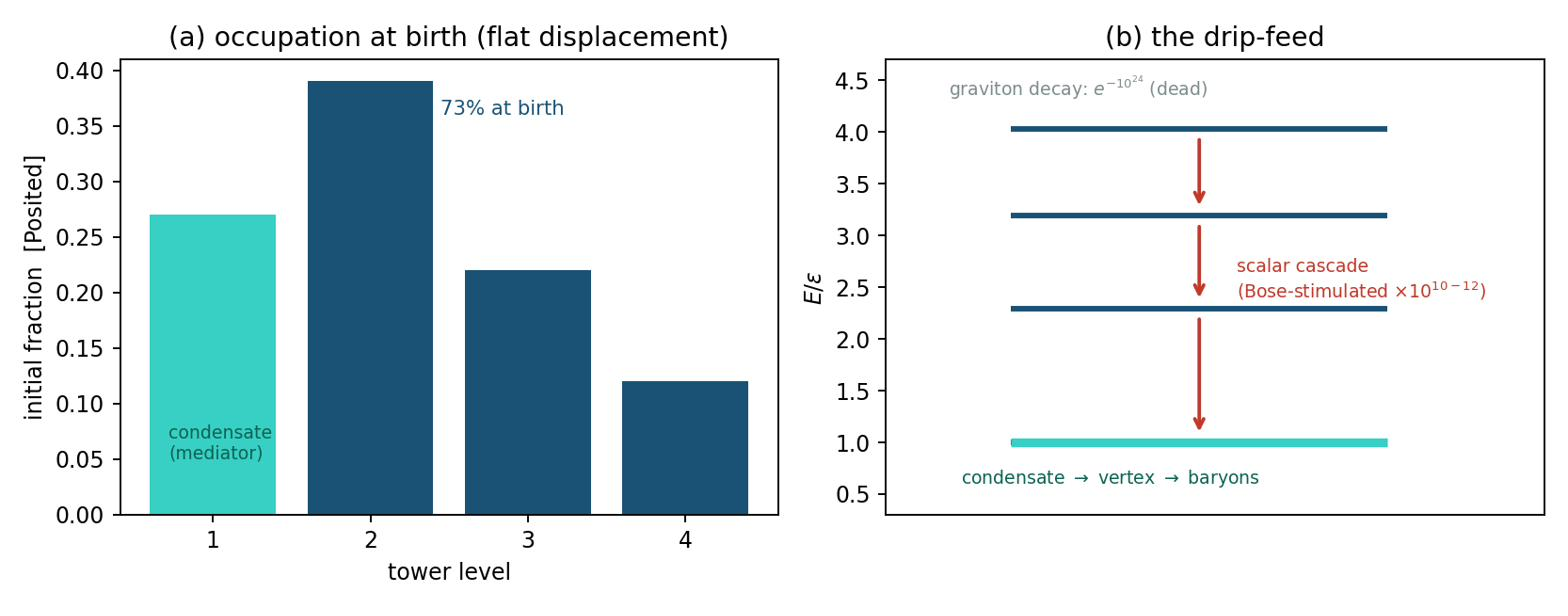
\includegraphics[width=0.95\textwidth]{fig1_medium.png}
\caption{The medium. (a) Occupation at birth for the flat displacement [Posited]: the upper floors carry $73\%$ --- the reservoir dominates from the start. (b) The drip-feed: graviton decay is dead ($e^{-10^{24}}$); the scalar cascade, stimulated by the reservoir's Bose degeneracy ($n\lambda_{\rm dB}^{3}\sim10^{10\text{--}12}$), trickles energy to the ground-state condensate, which the boundary vertex couples to the baryons. [\texttt{medium\_numbers.py}]}
\label{fig:medium}
\end{figure}

\section{The response, and a null that arrived as a prediction}
The condensate answers the baryons through the single boundary vertex of Article I, with the closed amplitude of Article II, $\alpha_{b}=3.3\,c_{b}$: a phonon-mediated attraction that \emph{adds} to gravity wherever the medium is coherent. Superposed on the Newtonian field of the disc, the addition reproduces the radial-acceleration relation of galaxies --- the tight, regular correlation between observed and baryonic acceleration that pure particle dark matter must arrange halo by halo, and that here is the medium's response law, one amplitude for all galaxies. In the coherent region the total acceleration follows
\begin{equation}
g_{\rm obs}\;=\;g_{\rm bar}+g_{\rm med},\qquad g_{\rm med}\;\xrightarrow[g_{\rm bar}\ll g_{\dagger}]{}\;\sqrt{g_{\dagger}\,g_{\rm bar}}\,,
\end{equation}
the phonon-mediated pull interpolating to the deep-regime square-root that the data demand, with the single response scale $g_{\dagger}$ set by the amplitude $\alpha_{b}$ and the medium --- not per galaxy. The dossier pipeline returns $g_{\dagger}=9.3\times10^{-11}$~m\,s$^{-2}$ on the full SPARC sample at the standard mass-to-light ratio, against $1.2\times10^{-10}$ in the literature's original fit: one number, every galaxy. The requirement that it hold across the SPARC sample is what fixed the benchmark amplitudes translated into $c_{b}=0.30$--$0.61$ in Article II. [Derived response; amplitude from the closed accounting]

Because the response needs coherence, it switches off where coherence dies (\S5) --- and this yields the framework's cleanest confirmed prediction. Wide stellar binaries beyond $\sim$10~kau live inside the decoherence bubbles of their own stars: the framework requires them \emph{Newtonian}, precisely where modified-dynamics accounts with an external-field effect expect an enhancement of order $\sqrt{1.4}$. Independent analysis of the Gaia DR3 pairs returns $\gamma=G_{\rm eff}/G=1.00$--$1.05$, with the modified-dynamics value excluded at high significance [measurement companion]. The null result that is a difficulty elsewhere arrives here on schedule: the switch is not a loophole, it is the mechanism, observed. [Prediction, confirmed]

\section{Decoherence and the condensed fraction}
\subsection{The off-switch, quantified}
A condensate survives only where the gravitational environment does not scramble its phase. Around any mass concentration $M$ in a background of density $\rho$, coherence dies within
\begin{equation}
R_{\rm dec}\;=\;K\,\frac{(M/\Msun)^{1/3}}{f\,\rho}\,,\qquad K=4.9\times10^{-4}~\mathrm{pc\cdot GeV\,cm^{-3}},
\label{eq:rdec}
\end{equation}
with $f$ the local condensed fraction; the single constant $K$ is fixed once by the medium's microphysics, and the $M^{1/3}$ scaling --- the tidal-granularity law --- was adopted after the framework's derivation programme tested it against its alternative. [Derived form; one constant]
\subsection{The fraction is measured, and it flows}
The condensed fraction is bounded on both sides: from below by demanding coherence across the interstellar volume (or the response would die everywhere), and from above by the wide-binary switch of \S4 --- with the upper jaw since tightened twice --- by the kinematics of the gas-rich ultra-diffuse galaxy AGC~114905, then by the 30~kau wide-binary null of the estimator-forensics companion (arXiv:2608.24556) --- giving
\begin{equation}
f\in[1.2\times10^{-3},\;8.42\times10^{-3}] .
\end{equation}
One structural statement accompanies the number: the condensate \emph{flows}. A superfluid ground state does not sit in a halo profile of its own; it relaxes toward uniform fraction across the coherent volume --- which is what the universality of the response law demands, since a patchy $f$ would scatter the radial-acceleration relation that observation shows tight. The framework's judge here forced its hydrodynamics. And the same switch explains the sky's strangest dwarf: NGC1052--DF2, the galaxy ``missing dark matter's gravity boost'', sits in a high-density, high-tide environment where Eq.~(\ref{eq:rdec}) predicts decoherence --- the medium is present but silent, and the galaxy shows only its baryons and its reservoir. [Measured window; flow forced by the RAR; DF2 explained]

\section{Where the response is off}
\emph{Clusters, at two tiers.} The first tier is parameter-free: at least $98.6\%$ of the dark sector is particulate reservoir whatever the phase (\S1), so cluster lensing and dynamics are carried by collisionless mass exactly as cold dark matter would carry them --- \textbf{cluster masses are cluster masses, by mass budget alone}, and the lensing-mass difficulty of pure modified dynamics is not inherited; the Bullet Cluster's lensing tracks the reservoir. The second tier concerns the medium's own phase inside clusters, and one scaling is there \emph{declared} rather than assumed --- with the conclusion insensitive to the declaration: in the cluster environment the mediated addition is absent either because the medium is decoherent or because it is light, and the sub-percent mediator budget cannot change a cluster mass in any case. [Tier one: Derived; tier two: declared, conclusion insensitive]

\emph{The Solar System, for free.} Inserting the Sun in the local environment into Eq.~(\ref{eq:rdec}) gives a decoherence bubble of at least $\sim$30~kau (at the largest allowed $f$; a parsec at the smallest) --- vastly beyond Saturn. Inside the bubble the response channel is switched off: the post-Newtonian metric is that of general relativity, and the Cassini bound $\gamma-1\lesssim2\times10^{-5}$ is met \emph{identically} rather than approximately, with a factor of a thousand in radius to spare. The transition at the bubble edge is smooth on the condensate's healing length --- a microphysical width set by the medium itself, far below any orbital scale, and not a new parameter --- so no discontinuity propagates into the ephemerides. Planetary tests constrain nothing here because there is nothing present to constrain: the framework passes them for free, by the same switch that the wide binaries confirmed. [Derived]

\section{Universality, bounded by data}
The covariant vertex couples the medium to the \emph{trace} of the baryonic stress tensor, so a composition dependence of the response is expected at the level of binding-energy differences --- of order $0.7\%$ between gas and stars. Locally the question is screened (the bubble contains no medium to respond), so the test is galactic: do gas-dominated and star-dominated galaxies obey the same response law? This article answers with the first quantitative bound. Across 171 SPARC galaxies, fitting the response scale per population with the stellar mass-to-light ratio $\Upsilon$ marginalised --- the decisive step, since $\Upsilon$ enters the baryonic acceleration of star-dominated galaxies only, and any error in it forges a spurious composition signal --- the result is
\begin{equation}
\left|\frac{\Delta\alpha_{b}}{\alpha_{b}}\right|\;\leq\;9\%\ \ \text{at}\ \Upsilon_{\star}=0.5\ (p=0.08),\qquad \leq\;14\%\ \ \text{over}\ \Upsilon_{\star}\in[0.4,0.8].
\end{equation}
The degeneracy is declared rather than hidden, and its structure must be stated precisely. The bound is not a measurement of the composition dependence; it is the envelope that survives a marginalised fit in which the stellar mass-to-light ratio is free. The apparent offset crosses zero at $\Upsilon_{\star}=0.69$, within $2\sigma$ of the population-synthesis standard, which means that present data cannot distinguish two hypotheses: (i) a small composition effect of the covariant vertex, and (ii) a small recalibration of the stellar mass-to-light ratio. The bound is what survives that honesty. It sits an order of magnitude above the predicted $0.7\%$: compatible with the framework, not yet a test of it. What would convert the bound into a test is an independent determination of $\Upsilon_{\star}$, obtained without reference to the dynamical mass that the response law itself predicts. Three routes are available: resolved stellar populations (counting stars rather than weighing light), vertical dynamics of the disc (the restoring force per unit mass, independent of the luminosity), and gravitational lensing (the total mass, independent of its composition). Any one of these, applied to the SPARC sample or a comparable one, fixes $\Upsilon_{\star}$ independently and converts the degeneracy into a measurement. Until then, the bound stands as the honest limit of present data --- a measurement target, not a verdict. Universality, long an open structural assumption of media-based frameworks, is here a number with an error bar, set by the data, not by the theory. [Measured bound; methodology in Appendix~A]

\begin{figure}[t]
\centering
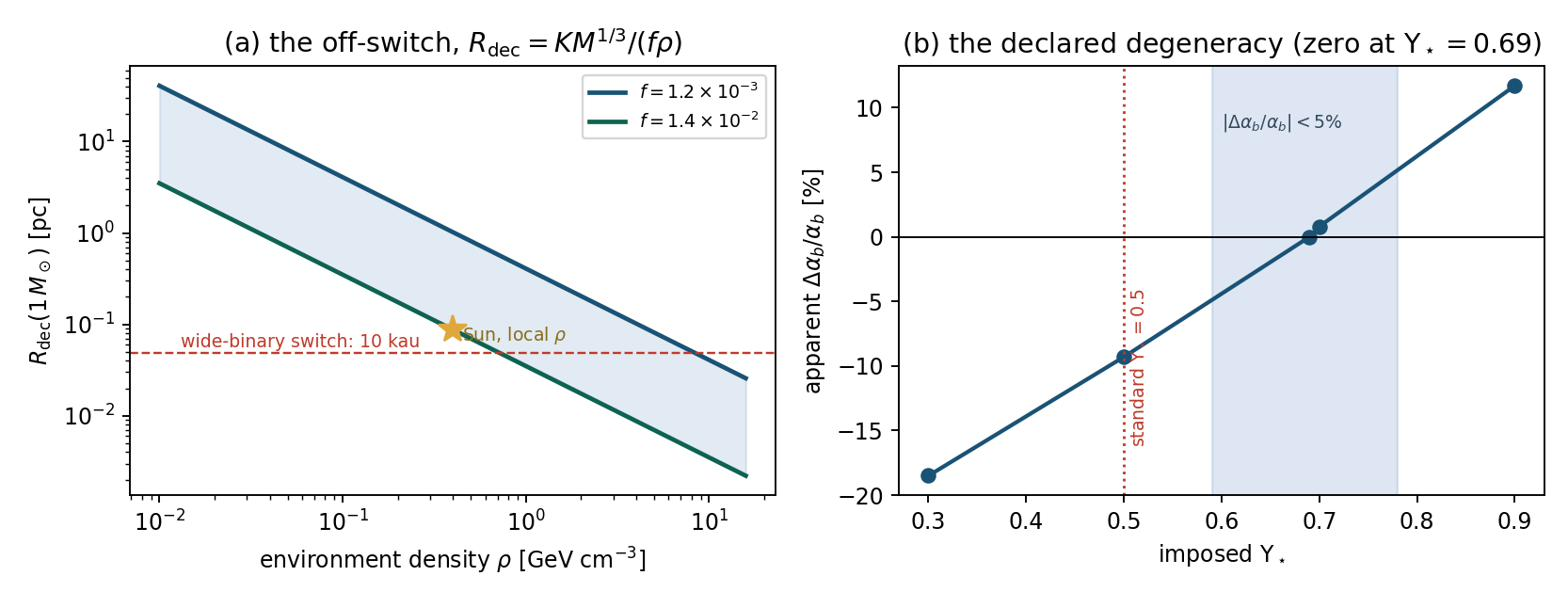
\includegraphics[width=0.95\textwidth]{fig2_switch.png}
\caption{The off-switch and the universality bound. (a) Decoherence radius around a solar-mass star versus environment density, for the measured $f$ window: the Solar System's bubble spans $\sim$0.09--1~pc --- Cassini is inside by a factor $\gtrsim10^{3}$; wide binaries beyond 10~kau are inside their hosts' bubbles (Newtonian, as observed); the interstellar medium at large is outside (response on). (b) The apparent composition offset versus the assumed $\Upsilon_{\star}$ (points from the dossier analysis): zero-crossing at $0.69$, within $2\sigma$ of the standard --- the declared degeneracy behind the $9$--$14\%$ bound. [\texttt{medium\_numbers.py}, \texttt{C4\_run\_sparc.py} + \texttt{03\_data/sparc\_3375\_points.csv}]}
\label{fig:switch}
\end{figure}

\section{How this article dies}
(i) \emph{The permanent judge:} any future tightening of the Bullet-type self-interaction ceiling below the stimulated floor closes the $\lambda$ window and stops the drip. (ii) \emph{The switch, both ways:} isolated ultra-diffuse galaxies showing a mediated boost where Eq.~(\ref{eq:rdec}) predicts coherence would be fine --- but a boost \emph{inside} a predicted bubble (or Gaia DR4 wide binaries departing from $\gamma=1$ within the decoherence edge) breaks the mechanism that \S4 celebrated; the framework has pre-registered this test for the DR4 sample. (iii) \emph{A patchy response:} significant galaxy-to-galaxy scatter of the response amplitude at fixed environment contradicts the flowing condensate. (iv) \emph{Universality:} a composition dependence confirmed above $\sim$1\% with an independent $\Upsilon_{\star}$ exceeds the covariant vertex's budget and falsifies the coupling structure; conversely, an independent $\Upsilon_{\star}$ that moves the bound below the predicted $0.7\%$ would confirm the vertex at the level the framework expects --- both outcomes are scheduled by the data, and the framework does not choose between them. (v) \emph{A warm sector:} any CMB evidence of dark reheating breaks the cold deposition. Article IV now steps back from the machinery and states what the framework \emph{is}: one scale, its shadow, and the map of everything this series has claimed, declared, or left to the sky.

\appendix
\section{The universality analysis}
The bound of \S7 was produced by the dossier pipeline (\texttt{C4\_run\_sparc.py} on \texttt{sparc\_3375\_points.csv}; 171 galaxies, 3375 points) in three steps designed against the known failure modes. \emph{Reference:} the radial-acceleration relation itself, fitted as $g_{\rm obs}=g_{\rm bar}/(1-e^{-\sqrt{g_{\rm bar}/g_{\dagger}}})$ with the response scale $g_{\dagger}$ free --- never a pre-fitted global model, whose residuals would contaminate the comparison (the pipeline's sanity checks return $g_{\dagger}=9.3\times10^{-11}$~m\,s$^{-2}$ globally at $\Upsilon_{\star}=0.5$, and a best-fit $\Upsilon_{\star}=0.56$, both in the literature's range). \emph{Populations:} galaxies split by outer gas fraction at thresholds 0.3--0.7, with $g_{\dagger}$ fitted per population and the composition signal read as $\Delta\alpha_{b}/\alpha_{b}=\tfrac{1}{2}\,\Delta g_{\dagger}/g_{\dagger}$ (the deep-regime translation). \emph{Marginalisation and errors:} $\Upsilon_{\star}$ is fitted on the star-dominated population alone --- the gas-rich one is insensitive to it, which is what breaks the degeneracy as far as SPARC allows --- and significance is assessed by bootstrap over \emph{galaxies}, not points, since the points of one rotation curve are correlated (per-point statistics overstate significance several-fold). The scan of the apparent offset against an imposed $\Upsilon_{\star}$ (Fig.~\ref{fig:switch}b) makes the residual degeneracy explicit; the quoted bound is the envelope over thresholds and over $\Upsilon_{\star}\in[0.4,0.8]$. The analysis is reproducible from the shipped CSV in one command.


% ═══════════════════════════════════════════════════════════════════════════
%  APPENDICE DE LIAISON — identique dans les sept articles.
%  % ═══════════════════════════════════════════════════════════════════════════
%  APPENDICE DE LIAISON — identique dans les sept articles.
%  % ═══════════════════════════════════════════════════════════════════════════
%  APPENDICE DE LIAISON — identique dans les sept articles.
%  \input{appendix-where} juste avant \begin{thebibliography} ou la biblio.
%  Il répond à : qui vit où, et qu'est-ce que la série a changé en cours de route.
% ═══════════════════════════════════════════════════════════════════════════
\section*{Appendix: which sector lives where, and what changed}
\addcontentsline{toc}{section}{Appendix: which sector lives where}

The series was written over several months and \textbf{two of its assignments moved}.
A reader who meets the articles out of order is owed an explicit map rather than an
inference, so it is given here, identically in all seven papers.

\subsection*{A.1 The three locations}
The geometry has three places where physics can sit: the \emph{brane} at $y=0$,
the \emph{bulk} of the $8.2\,\mu$m interval, and the \emph{far wall} at $y=\pi R$.
\begin{center}\small
\begin{tabular}{llll}\toprule
sector & lives on & carried by & established in\\\midrule
ordinary matter & \textbf{brane} & thin core, Standard Model & I\\
gravity, radion, graviton & \textbf{bulk} & five-dimensional fields & I\\
the mediator $\Phi$ and its tower & \textbf{bulk} & Airy states of the $|y|$ well & II\\
the galactic response & \textbf{bulk} $\to$ brane & $\Phi$ exchange between baryons & III\\
dark matter & \textbf{see A.2} & --- & III, revisited in VI\\
dark energy & \textbf{see A.3} & --- & III, revisited in VI\\
hidden gauge sector & \textbf{far wall} & eight D8 and one O8 & V\\\bottomrule
\end{tabular}
\end{center}

\subsection*{A.2 Dark matter: the reservoir, and what the wall reading adds}
Articles~I--IV place dark matter in the \emph{bulk}: the excited states of the Airy
tower, populated cold at birth, collisionless, carrying at least $98.6\%$ of the dark
sector's density. That assignment does the work in three places. It makes structure
formation identical to cold dark matter at linear order. It answers the Bullet Cluster
by mass budget alone --- cluster masses are cluster masses, and the lensing tracks the
reservoir, which is why the lensing--dynamics difficulty of purely modified dynamics is
not inherited. And it fixes the radiation budget of Article~I.

Article~VI proposes a different reading: dark matter as the ordinary matter of the six
other regions of the same wall, seen through the bulk, giving
$\Omega_{\rm DM}/\Omega_b=N_{\rm regions}-1=6$ against an observed $5.31$.
\textbf{These are not the same statement, and we do not pretend otherwise.}

What they share is everything the phenomenology uses: in both readings the dark
component is cold, collisionless, and carries the mass, so lensing, the Bullet Cluster
and linear structure formation are unaffected. What differs is the \emph{constituent}:
quanta of $\Phi$ in the first, baryons of other regions in the second.
\textbf{The two are compatible if the tower reservoir is not required to be the whole
of the dark matter} --- and Article~III's own argument only requires it to dominate the
budget, not to be exhaustive. \Open

\subsection*{A.3 Dark energy: a bulk scalar, then a brane curvature}
Articles~I--IV treat $\Phi$ as the dark-energy candidate --- a bulk scalar engine. That
attempt \emph{failed by forty orders of magnitude}: a four-dimensional scalar cannot
reach $2.4$~meV from a $10^{-13}$~eV engine scale. The failure is recorded, not hidden.

Article~VI relocates dark energy \emph{to the brane}, as the extrinsic curvature of the
D8 wall in the cosmological bulk, $\Lambda_4=\varepsilon^2(1/R)^4$ with
$\varepsilon\simeq10^{-2}$. The mechanism supplies $(1/R)^4$ outright and leaves a gap
of $10^4$ rather than $10^{40}$. \textbf{$\Phi$ is correspondingly demoted from
dark-energy candidate to dark-sector mediator}, which is the role Articles~II and III
already gave it in every equation they actually use. \Candidate, declared tuning.

\subsection*{A.4 The radial acceleration relation, and what makes galaxies turn}
The relation is the one place where brane and bulk are \emph{both} indispensable, and
where nothing has moved since Article~III.

Baryons sit on the brane. They source $\Phi$, which propagates in the bulk with mass
$m_\Phi=24$~meV and hence Compton range $8.2\,\mu$m --- microscopic, so no fifth force
acts between laboratory bodies. What acts at galactic scale is not the free field but
the \emph{medium}: the coherent component of the dark sector responds to the baryonic
distribution, and that response, read back on the brane, is the extra acceleration.
The response saturates, which is why it produces a relation --- an acceleration scale
$g_\dagger$ --- rather than a rescaling of Newton's constant.

Three consequences, all in Article~III and unchanged:
\begin{itemize}\itemsep2pt
\item the response couples to the trace $T^\mu_{\ \mu}$, hence to mass and not to
      composition; the universality is bounded on 171 SPARC galaxies;
\item the response is carried by at most $1.4\%$ of the dark sector, the coherent part,
      so it never competes with the reservoir in the mass budget --- \textbf{galaxies
      turn because of the medium, they weigh because of the reservoir};
\item the response \emph{dies} in weak field, which is the ultra-diffuse galaxy test,
      and it dies in a decoherence bubble around the Sun, which is why Cassini is
      satisfied identically rather than by tuning.
\end{itemize}
\textbf{Neither relocation of A.2 or A.3 touches this.} The galactic response was never
assigned to the dark-energy sector, and it is not the reservoir either; it is the third
role, and it is the one the framework was built to explain.

\subsection*{A.5 What a reader should carry between articles}
Articles~I--IV stand on their own evidence and are not modified by V--VII: no result of
theirs is derived from the string embedding, and the embedding cannot promote any of
their labels. What V--VII add is an ultraviolet origin for one constant, a candidate
geometry, and two consequences of that geometry. What they \emph{change} is recorded
above and nowhere else: two relocations, both declared, neither retroactive.
 juste avant \begin{thebibliography} ou la biblio.
%  Il répond à : qui vit où, et qu'est-ce que la série a changé en cours de route.
% ═══════════════════════════════════════════════════════════════════════════
\section*{Appendix: which sector lives where, and what changed}
\addcontentsline{toc}{section}{Appendix: which sector lives where}

The series was written over several months and \textbf{two of its assignments moved}.
A reader who meets the articles out of order is owed an explicit map rather than an
inference, so it is given here, identically in all seven papers.

\subsection*{A.1 The three locations}
The geometry has three places where physics can sit: the \emph{brane} at $y=0$,
the \emph{bulk} of the $8.2\,\mu$m interval, and the \emph{far wall} at $y=\pi R$.
\begin{center}\small
\begin{tabular}{llll}\toprule
sector & lives on & carried by & established in\\\midrule
ordinary matter & \textbf{brane} & thin core, Standard Model & I\\
gravity, radion, graviton & \textbf{bulk} & five-dimensional fields & I\\
the mediator $\Phi$ and its tower & \textbf{bulk} & Airy states of the $|y|$ well & II\\
the galactic response & \textbf{bulk} $\to$ brane & $\Phi$ exchange between baryons & III\\
dark matter & \textbf{see A.2} & --- & III, revisited in VI\\
dark energy & \textbf{see A.3} & --- & III, revisited in VI\\
hidden gauge sector & \textbf{far wall} & eight D8 and one O8 & V\\\bottomrule
\end{tabular}
\end{center}

\subsection*{A.2 Dark matter: the reservoir, and what the wall reading adds}
Articles~I--IV place dark matter in the \emph{bulk}: the excited states of the Airy
tower, populated cold at birth, collisionless, carrying at least $98.6\%$ of the dark
sector's density. That assignment does the work in three places. It makes structure
formation identical to cold dark matter at linear order. It answers the Bullet Cluster
by mass budget alone --- cluster masses are cluster masses, and the lensing tracks the
reservoir, which is why the lensing--dynamics difficulty of purely modified dynamics is
not inherited. And it fixes the radiation budget of Article~I.

Article~VI proposes a different reading: dark matter as the ordinary matter of the six
other regions of the same wall, seen through the bulk, giving
$\Omega_{\rm DM}/\Omega_b=N_{\rm regions}-1=6$ against an observed $5.31$.
\textbf{These are not the same statement, and we do not pretend otherwise.}

What they share is everything the phenomenology uses: in both readings the dark
component is cold, collisionless, and carries the mass, so lensing, the Bullet Cluster
and linear structure formation are unaffected. What differs is the \emph{constituent}:
quanta of $\Phi$ in the first, baryons of other regions in the second.
\textbf{The two are compatible if the tower reservoir is not required to be the whole
of the dark matter} --- and Article~III's own argument only requires it to dominate the
budget, not to be exhaustive. \Open

\subsection*{A.3 Dark energy: a bulk scalar, then a brane curvature}
Articles~I--IV treat $\Phi$ as the dark-energy candidate --- a bulk scalar engine. That
attempt \emph{failed by forty orders of magnitude}: a four-dimensional scalar cannot
reach $2.4$~meV from a $10^{-13}$~eV engine scale. The failure is recorded, not hidden.

Article~VI relocates dark energy \emph{to the brane}, as the extrinsic curvature of the
D8 wall in the cosmological bulk, $\Lambda_4=\varepsilon^2(1/R)^4$ with
$\varepsilon\simeq10^{-2}$. The mechanism supplies $(1/R)^4$ outright and leaves a gap
of $10^4$ rather than $10^{40}$. \textbf{$\Phi$ is correspondingly demoted from
dark-energy candidate to dark-sector mediator}, which is the role Articles~II and III
already gave it in every equation they actually use. \Candidate, declared tuning.

\subsection*{A.4 The radial acceleration relation, and what makes galaxies turn}
The relation is the one place where brane and bulk are \emph{both} indispensable, and
where nothing has moved since Article~III.

Baryons sit on the brane. They source $\Phi$, which propagates in the bulk with mass
$m_\Phi=24$~meV and hence Compton range $8.2\,\mu$m --- microscopic, so no fifth force
acts between laboratory bodies. What acts at galactic scale is not the free field but
the \emph{medium}: the coherent component of the dark sector responds to the baryonic
distribution, and that response, read back on the brane, is the extra acceleration.
The response saturates, which is why it produces a relation --- an acceleration scale
$g_\dagger$ --- rather than a rescaling of Newton's constant.

Three consequences, all in Article~III and unchanged:
\begin{itemize}\itemsep2pt
\item the response couples to the trace $T^\mu_{\ \mu}$, hence to mass and not to
      composition; the universality is bounded on 171 SPARC galaxies;
\item the response is carried by at most $1.4\%$ of the dark sector, the coherent part,
      so it never competes with the reservoir in the mass budget --- \textbf{galaxies
      turn because of the medium, they weigh because of the reservoir};
\item the response \emph{dies} in weak field, which is the ultra-diffuse galaxy test,
      and it dies in a decoherence bubble around the Sun, which is why Cassini is
      satisfied identically rather than by tuning.
\end{itemize}
\textbf{Neither relocation of A.2 or A.3 touches this.} The galactic response was never
assigned to the dark-energy sector, and it is not the reservoir either; it is the third
role, and it is the one the framework was built to explain.

\subsection*{A.5 What a reader should carry between articles}
Articles~I--IV stand on their own evidence and are not modified by V--VII: no result of
theirs is derived from the string embedding, and the embedding cannot promote any of
their labels. What V--VII add is an ultraviolet origin for one constant, a candidate
geometry, and two consequences of that geometry. What they \emph{change} is recorded
above and nowhere else: two relocations, both declared, neither retroactive.
 juste avant \begin{thebibliography} ou la biblio.
%  Il répond à : qui vit où, et qu'est-ce que la série a changé en cours de route.
% ═══════════════════════════════════════════════════════════════════════════
\section*{Appendix: which sector lives where, and what changed}
\addcontentsline{toc}{section}{Appendix: which sector lives where}

The series was written over several months and \textbf{two of its assignments moved}.
A reader who meets the articles out of order is owed an explicit map rather than an
inference, so it is given here, identically in all seven papers.

\subsection*{A.1 The three locations}
The geometry has three places where physics can sit: the \emph{brane} at $y=0$,
the \emph{bulk} of the $8.2\,\mu$m interval, and the \emph{far wall} at $y=\pi R$.
\begin{center}\small
\begin{tabular}{llll}\toprule
sector & lives on & carried by & established in\\\midrule
ordinary matter & \textbf{brane} & thin core, Standard Model & I\\
gravity, radion, graviton & \textbf{bulk} & five-dimensional fields & I\\
the mediator $\Phi$ and its tower & \textbf{bulk} & Airy states of the $|y|$ well & II\\
the galactic response & \textbf{bulk} $\to$ brane & $\Phi$ exchange between baryons & III\\
dark matter & \textbf{see A.2} & --- & III, revisited in VI\\
dark energy & \textbf{see A.3} & --- & III, revisited in VI\\
hidden gauge sector & \textbf{far wall} & eight D8 and one O8 & V\\\bottomrule
\end{tabular}
\end{center}

\subsection*{A.2 Dark matter: the reservoir, and what the wall reading adds}
Articles~I--IV place dark matter in the \emph{bulk}: the excited states of the Airy
tower, populated cold at birth, collisionless, carrying at least $98.6\%$ of the dark
sector's density. That assignment does the work in three places. It makes structure
formation identical to cold dark matter at linear order. It answers the Bullet Cluster
by mass budget alone --- cluster masses are cluster masses, and the lensing tracks the
reservoir, which is why the lensing--dynamics difficulty of purely modified dynamics is
not inherited. And it fixes the radiation budget of Article~I.

Article~VI proposes a different reading: dark matter as the ordinary matter of the six
other regions of the same wall, seen through the bulk, giving
$\Omega_{\rm DM}/\Omega_b=N_{\rm regions}-1=6$ against an observed $5.31$.
\textbf{These are not the same statement, and we do not pretend otherwise.}

What they share is everything the phenomenology uses: in both readings the dark
component is cold, collisionless, and carries the mass, so lensing, the Bullet Cluster
and linear structure formation are unaffected. What differs is the \emph{constituent}:
quanta of $\Phi$ in the first, baryons of other regions in the second.
\textbf{The two are compatible if the tower reservoir is not required to be the whole
of the dark matter} --- and Article~III's own argument only requires it to dominate the
budget, not to be exhaustive. \Open

\subsection*{A.3 Dark energy: a bulk scalar, then a brane curvature}
Articles~I--IV treat $\Phi$ as the dark-energy candidate --- a bulk scalar engine. That
attempt \emph{failed by forty orders of magnitude}: a four-dimensional scalar cannot
reach $2.4$~meV from a $10^{-13}$~eV engine scale. The failure is recorded, not hidden.

Article~VI relocates dark energy \emph{to the brane}, as the extrinsic curvature of the
D8 wall in the cosmological bulk, $\Lambda_4=\varepsilon^2(1/R)^4$ with
$\varepsilon\simeq10^{-2}$. The mechanism supplies $(1/R)^4$ outright and leaves a gap
of $10^4$ rather than $10^{40}$. \textbf{$\Phi$ is correspondingly demoted from
dark-energy candidate to dark-sector mediator}, which is the role Articles~II and III
already gave it in every equation they actually use. \Candidate, declared tuning.

\subsection*{A.4 The radial acceleration relation, and what makes galaxies turn}
The relation is the one place where brane and bulk are \emph{both} indispensable, and
where nothing has moved since Article~III.

Baryons sit on the brane. They source $\Phi$, which propagates in the bulk with mass
$m_\Phi=24$~meV and hence Compton range $8.2\,\mu$m --- microscopic, so no fifth force
acts between laboratory bodies. What acts at galactic scale is not the free field but
the \emph{medium}: the coherent component of the dark sector responds to the baryonic
distribution, and that response, read back on the brane, is the extra acceleration.
The response saturates, which is why it produces a relation --- an acceleration scale
$g_\dagger$ --- rather than a rescaling of Newton's constant.

Three consequences, all in Article~III and unchanged:
\begin{itemize}\itemsep2pt
\item the response couples to the trace $T^\mu_{\ \mu}$, hence to mass and not to
      composition; the universality is bounded on 171 SPARC galaxies;
\item the response is carried by at most $1.4\%$ of the dark sector, the coherent part,
      so it never competes with the reservoir in the mass budget --- \textbf{galaxies
      turn because of the medium, they weigh because of the reservoir};
\item the response \emph{dies} in weak field, which is the ultra-diffuse galaxy test,
      and it dies in a decoherence bubble around the Sun, which is why Cassini is
      satisfied identically rather than by tuning.
\end{itemize}
\textbf{Neither relocation of A.2 or A.3 touches this.} The galactic response was never
assigned to the dark-energy sector, and it is not the reservoir either; it is the third
role, and it is the one the framework was built to explain.

\subsection*{A.5 What a reader should carry between articles}
Articles~I--IV stand on their own evidence and are not modified by V--VII: no result of
theirs is derived from the string embedding, and the embedding cannot promote any of
their labels. What V--VII add is an ultraviolet origin for one constant, a candidate
geometry, and two consequences of that geometry. What they \emph{change} is recorded
above and nowhere else: two relocations, both declared, neither retroactive.

\toolsstatement
\traceability{3}{The reservoir occupation fractions, the cascade attractor and the galactic response are produced by \texttt{scripts/}.}
\bibliographystyle{unsrt}\bibliography{ddf-refs}

\section*{Appendix C: what the companion does, and does not, provide}
\addcontentsline{toc}{section}{Appendix C}
\label{app:companion}

A fifth article --- \emph{The Dark Dimension Framework from Type~I$'$ strings}, cited here as the companion --- asks whether the geometry of Articles~I--IV admits an ultraviolet completion. It is deposited together with this series so that a reader who asks \emph{where does this constant come from?} has somewhere to look. Three statements govern how it may be used.

\paragraph{It is a companion, not a foundation.} Every result, label and executioner of Articles~I--IV is established at the effective-theory level and stands or falls on its own evidence. If the companion's embedding is refuted tomorrow, nothing in this article changes. The converse also holds: the companion cannot promote a label here, and none of its findings has been used to do so.

\paragraph{What it establishes.} The companion shows that the framework's boundary conditions ($J_{0}+J_{\pi}=0$) are literally the Ramond--Ramond tadpole cancellation of a Type~I$'$ orientifold; it derives, at tree level, the coupling vector through which brane tension reaches the bulk scalar, obtaining three integer norm identities and an upper bound on the boundary constant, $c_{b}\leq\sqrt{255/56}=2.13$; it establishes two autonomous negative results (five independent moduli-pinning mechanisms fail, and massive type~IIA is incompatible with a mesoscopic interval); and it exhibits one explicit candidate vacuum that passes every computable test. For the present article there is no point of contact: the companion addresses the ultraviolet origin of the boundary vertex, not the medium's two roles, and none of the results of \S\S3--7 depends on it.

\paragraph{What it does not establish.} It does not derive the value of $c_{b}$. That value depends on the mixing angle of the light modulus, which in turn depends on string-loop coefficients that are not computable for a general Calabi--Yau manifold --- a frontier of that field, not of this construction. The companion therefore closes with a conditional statement, not a number. \textbf{Accordingly, no label in Articles~I--IV is altered by it}: what was [Input, natural] remains so, and what was [Open, declared] remains open.

\end{document}